% ===================================
% FIGURA 2.1 - Modello Tridimensionale Vulnerabilità
% Con posizionamento assoluto
% ===================================
\documentclass[tikz,border=10pt]{standalone}
\usepackage[T1]{fontenc}
\usepackage{tikz}
\usepackage{pgfplots}
\pgfplotsset{compat=1.17}
\usetikzlibrary{patterns}

\begin{document}
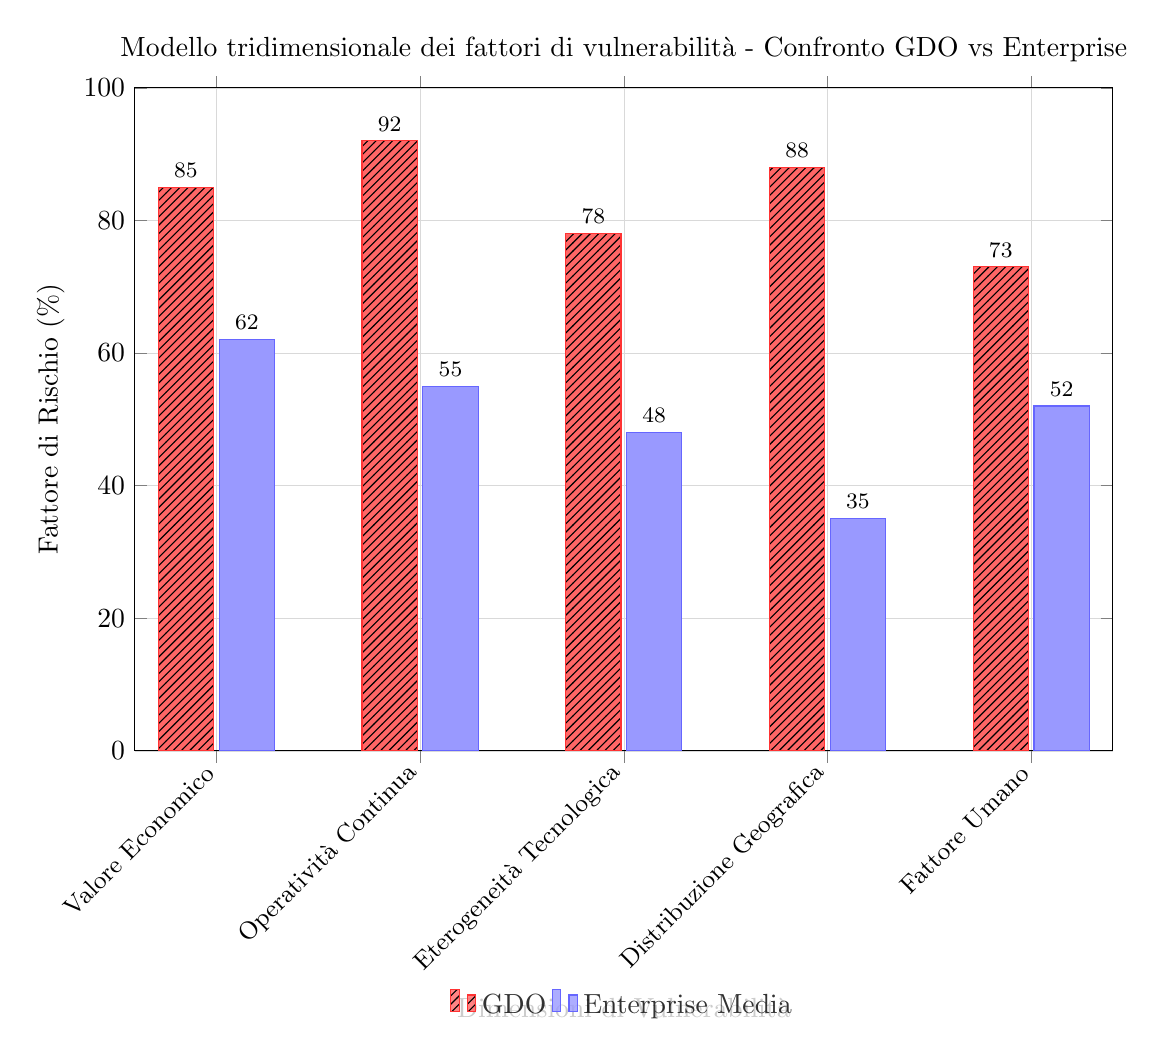
\begin{tikzpicture}
\begin{axis}[
    ybar,
    width=14cm,
    height=10cm,
    bar width=20pt,
    ylabel={Fattore di Rischio (\%)},
    xlabel={Dimensioni di Vulnerabilità},
    symbolic x coords={
        Valore Economico,
        Operatività Continua,
        Eterogeneità Tecnologica,
        Distribuzione Geografica,
        Fattore Umano
    },
    xtick=data,
    x tick label style={rotate=45, anchor=east, font=\small},
    ymin=0,
    ymax=100,
    grid=major,
    grid style={line width=.1pt, draw=gray!30},
    legend style={
        at={(0.5,-0.35)},
        anchor=north,
        legend columns=2,
        draw=none,
        fill=white,
        fill opacity=0.8
    },
    nodes near coords,
    every node near coord/.append style={font=\footnotesize},
    title={Modello tridimensionale dei fattori di vulnerabilità - Confronto GDO vs Enterprise}
]

% GDO
\addplot[
    fill=red!60,
    draw=red!80,
    postaction={pattern=north east lines}
] coordinates {
    (Valore Economico,85)
    (Operatività Continua,92)
    (Eterogeneità Tecnologica,78)
    (Distribuzione Geografica,88)
    (Fattore Umano,73)
};

% Enterprise Media
\addplot[
    fill=blue!40,
    draw=blue!60
] coordinates {
    (Valore Economico,62)
    (Operatività Continua,55)
    (Eterogeneità Tecnologica,48)
    (Distribuzione Geografica,35)
    (Fattore Umano,52)
};

\legend{GDO, Enterprise Media}

\end{axis}
\end{tikzpicture}
\end{document}